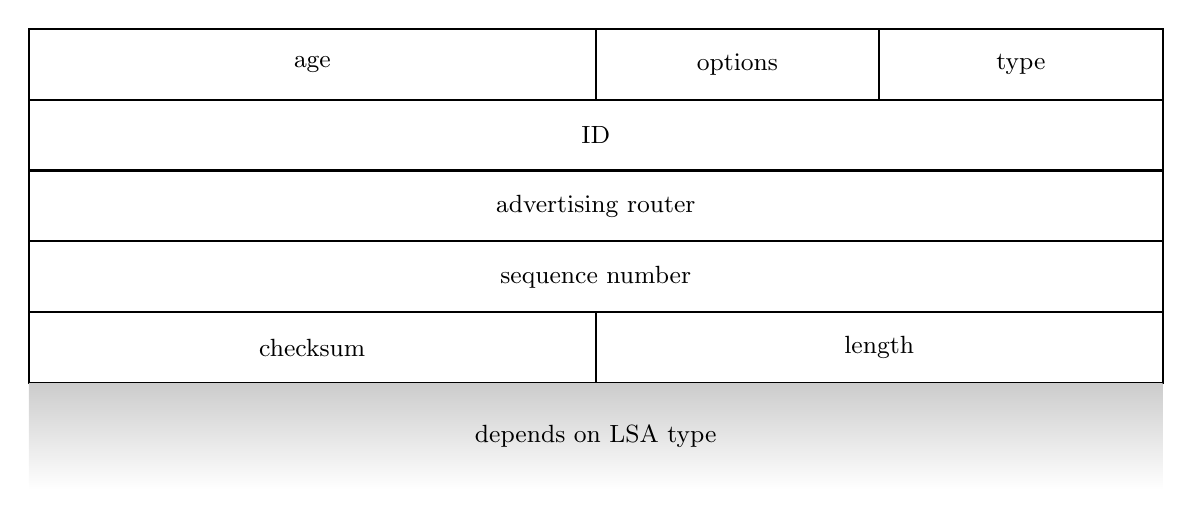
\begin{tikzpicture}
\tikzset{
    box/.style={draw,thick},
    label/.style={font=\small},
    label large/.style={},
    box label/.style={midway,font=\small,align=center},
    box label flags/.style={midway,font=\fontsize{8}{9}\selectfont,align=center},
    missing/.style={pattern=north west lines},
}
\begin{scope}[x=0.45cm,y=0.9cm]
\draw[box] (0, 0) rectangle (16, -1)
    node[midway,label] {age};
\draw[box] (16, 0) rectangle (24, -1)
    node[midway,label] {options};
\draw[box] (24, 0) rectangle (32, -1)
    node[midway,label] {type};
\draw[box] (0, -1) rectangle (32, -2)
    node[midway,label] {ID};
\draw[box] (0, -2) rectangle (32, -3)
    node[midway,label] {advertising router};
\draw[box] (0, -3) rectangle (32, -4)
    node[midway,label] {sequence number};
\draw[box] (0, -4) rectangle (16, -5)
    node[midway,label] {checksum};
\draw[box] (16, -4) rectangle (32, -5)
    node[midway,label] {length};
\path[shading=axis,bottom color=white,top color=black!20] (0, -5) rectangle (32, -6.5)
    node[box label] {depends on LSA type};
\end{scope}
\end{tikzpicture}
